\documentclass[brazil,times]{abnt}
\usepackage[T1]{fontenc}
\usepackage[utf8]{inputenc}
\usepackage{url}
\usepackage{graphicx}
\usepackage[pdfborder={0 0 0}]{hyperref}
\usepackage{amssymb}
\usepackage{amsmath}
\usepackage[section]{placeins}
\usepackage{listingsutf8}
\makeatletter
\usepackage{babel}
\makeatother


\lstset{
	language=Octave,
	tabsize=2,
	inputencoding=utf8,
	basicstyle=\scriptsize,
	showspaces=false,
	showstringspaces=false,
	showtabs=false,
}

\begin{document}


\autor{Pedro Paulo Vezzá Campos}

\titulo{Métodos de Processamento de Imagens}

\comentario{Segundo exercício-programa apresentado para avaliação na disciplina
MAC0300, do curso de Bacharelado em Ciência da Computação, turma 45, da
Universidade de São Paulo, ministrada pelo professor Walter Figueiredo Mascarenhas.}

\instituicao{Departamento de Ciência da Computação \par Instituto de Matemática
e Estatística \par Universidade de São Paulo}

\local{São Paulo - SP, Brasil}

\data{\today}

\capa

\folhaderosto

\tableofcontents

\chapter{Introdução\label{cap:introducao}}
	Neste segundo exercício-programa de MAC0300 - Métodos Numéricos da Álgebra Linear foi pedido que implementássemos um programa que fosse capaz de aplicar diferentes métodos de processamento de imagens em tons de cinza. Neste relatório serão apresentados: Uma explicação e a implementação para cada um dos filtros pedidos no enunciado, testes realizados e, por fim, será feita apresentada uma conclusão sobre o EP.

%Explique suscintamente o processo utilizado na implementação de cada um dos filtros;

%Mostre, para cada um dos métodos solicitados, as imagens originais e as obtidas após o processamento.

%Descreva as vantagens e desvantagens de cada um dos métodos, tanto em relação ao desempenho computacional como em relação ao desempenho como filtro de imagem.
\chapter{Métodos de Processamento de Imagens}

	\section{Ajuste de Contraste - Equalização de Histograma}
		O processo de equalizar um histograma de uma imagem, isto é, tornar aproximadamente iguais as quantidades de cada um dos tons de cinza em uma imagem, é uma maneira computacionalmente simples de gerar imagens que tem, em geral, contrastes melhores que as originais.

		\subsection{Vantagens e desvantagens}
			Este método possui como vantagens o fato de geralmente produzir imagens com maior contraste. Isto acontece quando o primeiro plano e fundo da imagem são claros ou escuros. Após a equalização as diferenças nas tonalidades de ambos é mais exacerbada o que permite visualizar melhor diferentes detalhes. Por outro lado, imagens que já apresentam diferenças significativas nos tons de cinza não terão grandes ganhos após a equalização. Além disso, como este método não diferencia trechos da imagem, o método pode piorar a relação sinal/ruído da imagem já que ruidos antes pouco visíveis passam a ser mais evidenciados.
			O algoritmo para este método é bastante simples, como poderemos ver a seguir, e ainda a complexidade computacional é linear no tamanho da imagem e na quantidade de tons de cinza existentes, o que faz o método ser bastante utilizado na prática.
			
		\subsection{Implementação}
			A implementação deste método segue um algoritmo simples: Devemos primeiramente calcular o histograma da imagem original (\texttt{p}) e com ele produzir o histograma acumulado (\texttt{fda}). Com os valores mínimo e máximo de \texttt{fda} podemos utilizar a fórmula deduzida no enunciado do EP para $h_X (i)$ (No código, \texttt{h}) que produz um mapeamento entre um tom de cinza da imagem original e o tom de cinza na nova imagem equalizada. O último passo é realizar o mapeamento para determinar a nova imagem.


\begin{lstlisting}
function [imagem] = equalizar_histograma(imagem)
	m = rows(imagem);
	n = columns(imagem);
	p = zeros(256, 1);
	fda = zeros(256, 1);
	
	%Parte 1: Calculando o histograma
	for j = 1 : n
		for i = 1 : m
			p(imagem(i,j) + 1) += 1;
		endfor
	endfor
	
	%Parte 2: Calculando o histograma acumulado
	fda(1) = p(1);
	for i = 2 : 256
		fda(i) = fda(i - 1) + p(i);
	endfor
	
	fda_min = min(fda);
	fda_max = max(fda);
	
	%Parte 3: Calculando o mapeamento
	h = zeros(256,1);
	for i = 1 : 256
		h(i) = round((fda(i) - fda_min)/(m * n - fda_min) * 255);
	endfor
	
	%Parte 4: Realizando o mapeamento para gerar a nova imagem
	for j = 1 : n
		for i = 1 : m
			imagem(i, j) = h(imagem(i,j) + 1);
		endfor
	endfor
endfunction
\end{lstlisting}

		%Para o método de ajuste de contraste por equalização de histograma, apresente também os histogramas correspondentes às imagens original e processada.
		\subsection{Testes realizados}
			Para apresentar as mudanças no histograma e na aparência das imagens que o método causa são apresentadas dois exemplos de imagens antes e depois de aplicado o método tendo ao lado o respectivo histograma. Podemos ver como o histogramas novos são mais distribuídos ao longo do eixo das intensidades (Eixo x).
			
			\begin{table}[ht]
			\caption{Imagens antes e depois de aplicada a equalização e seus respectivos histogramas}
			\centering
			\begin{tabular}{|c|c|}
			\hline
			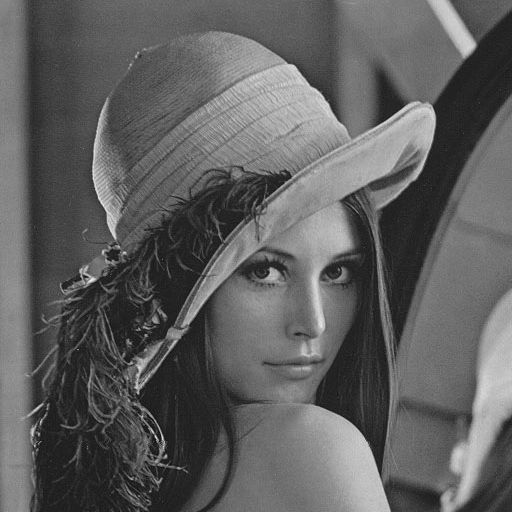
\includegraphics[scale=0.25]{imagens/lena.jpg}&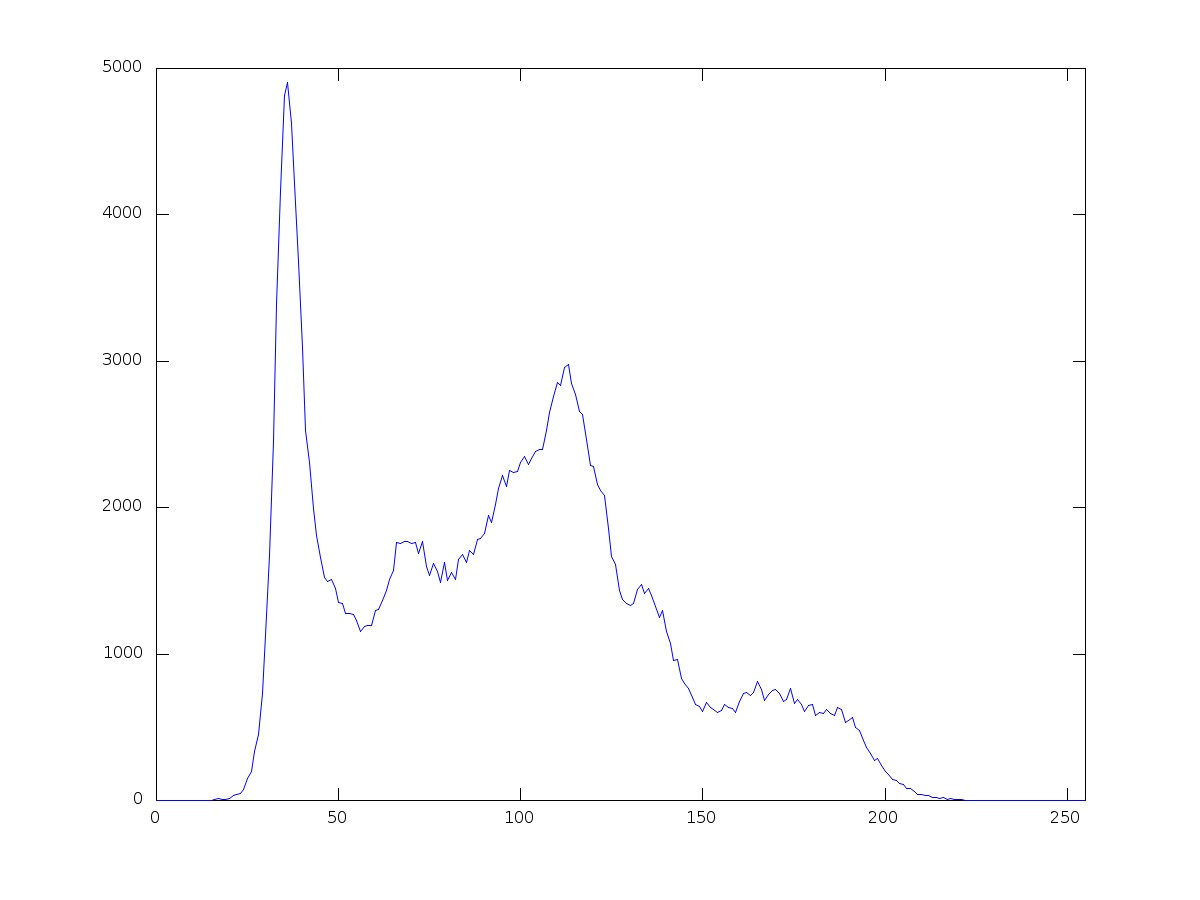
\includegraphics[scale=0.15]{imagens/lena-hist-original.jpg}\\
			\hline
			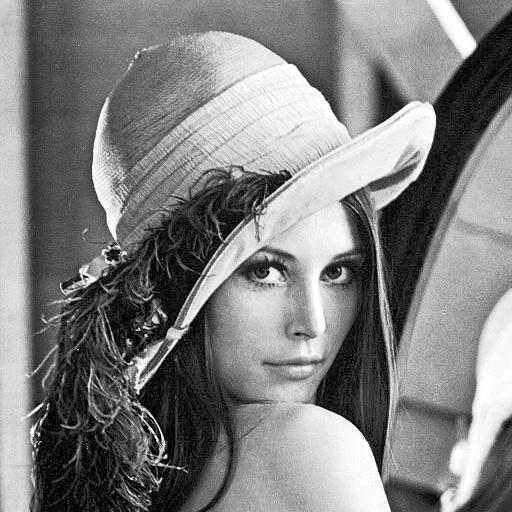
\includegraphics[scale=0.25]{imagens/lena-contrast.jpg}&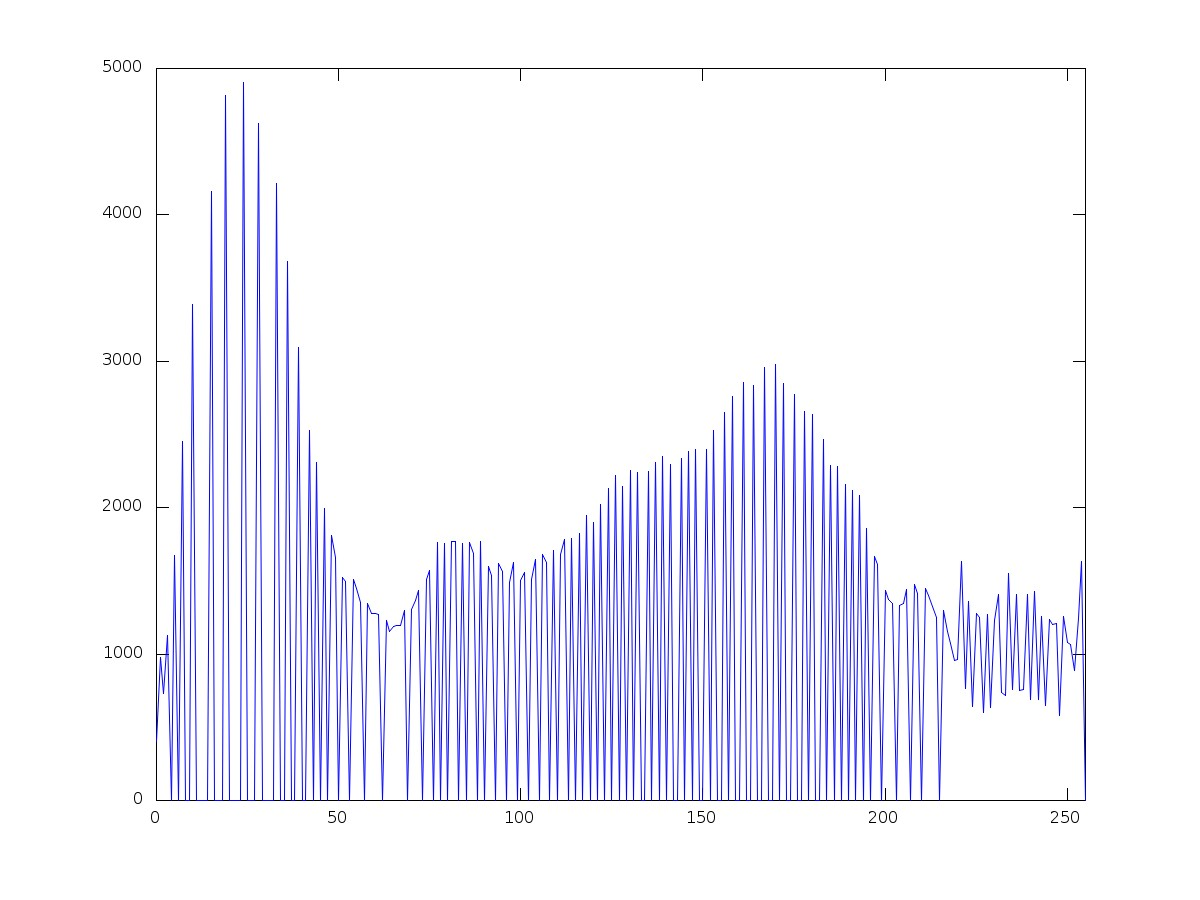
\includegraphics[scale=0.15]{imagens/lena-hist-novo.jpg}\\
			\hline
			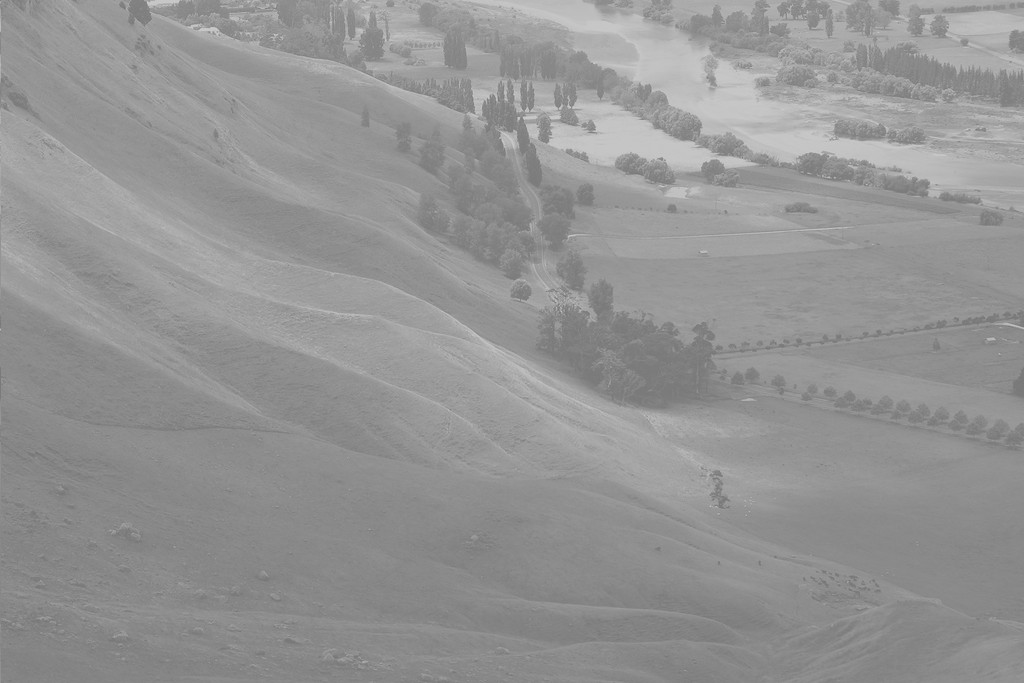
\includegraphics[scale=0.125]{imagens/hawkes.jpg}&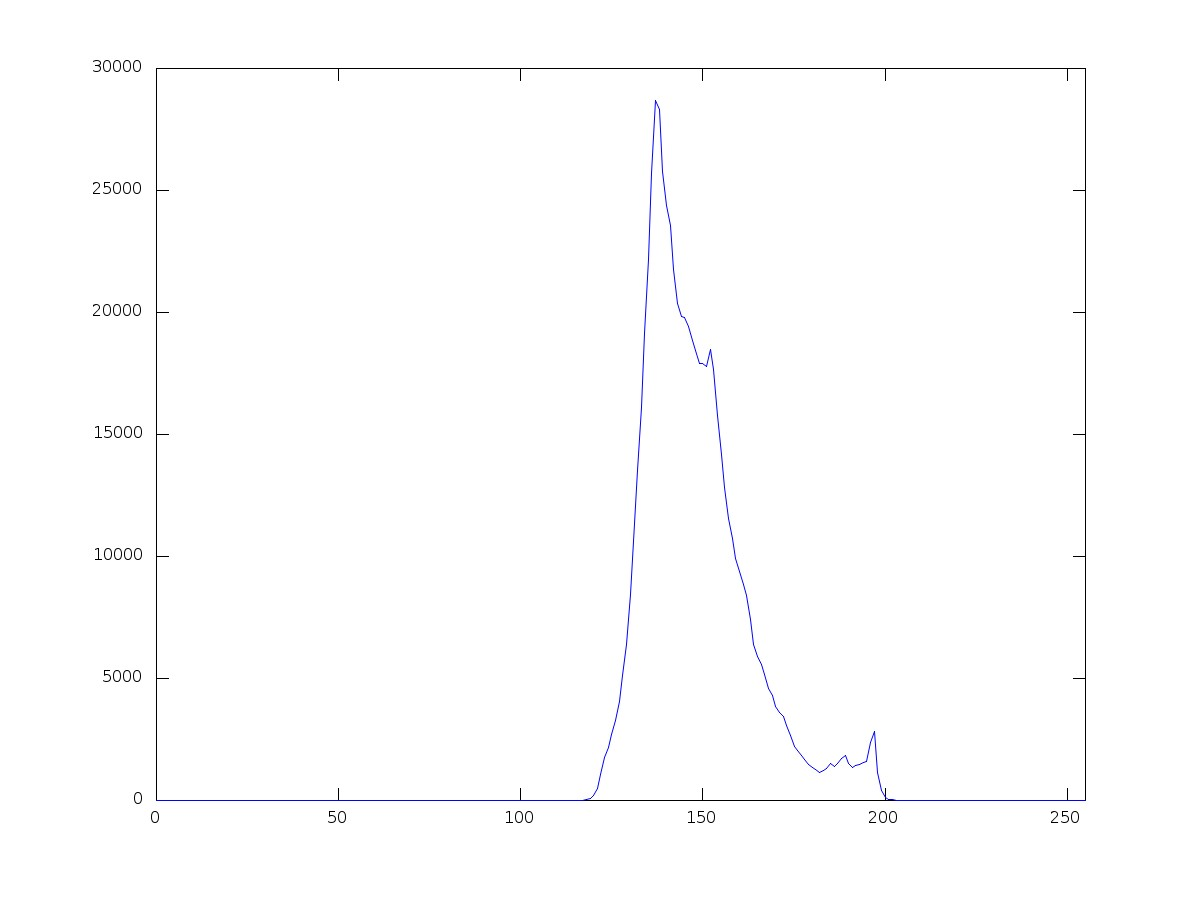
\includegraphics[scale=0.15]{imagens/hawkes-hist-original.jpg}\\
			\hline
			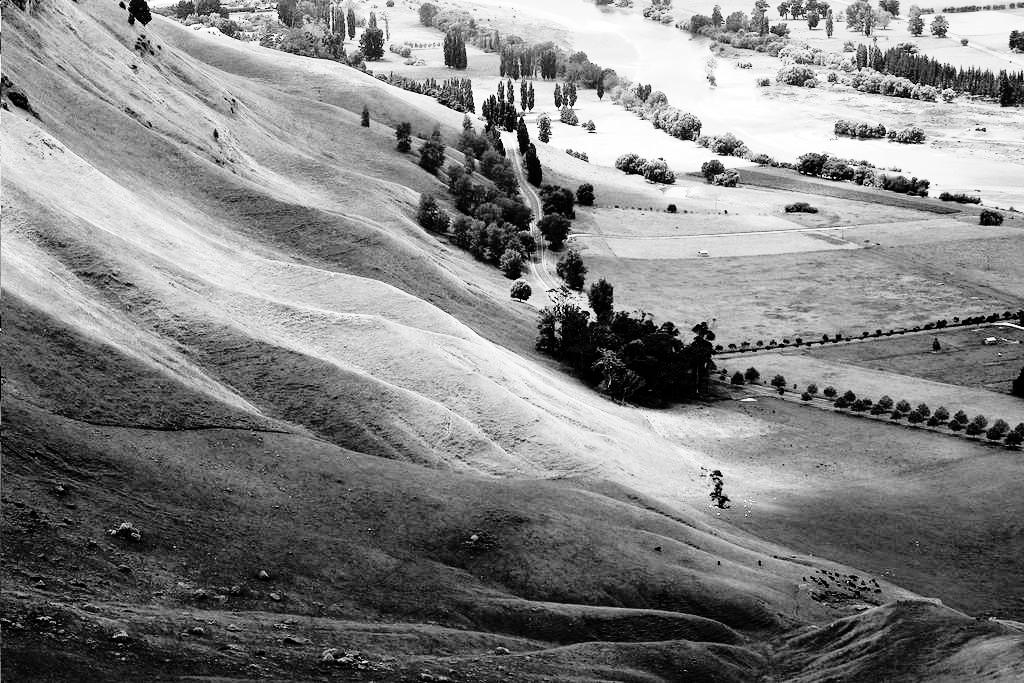
\includegraphics[scale=0.125]{imagens/hawkes-contrast.jpg}&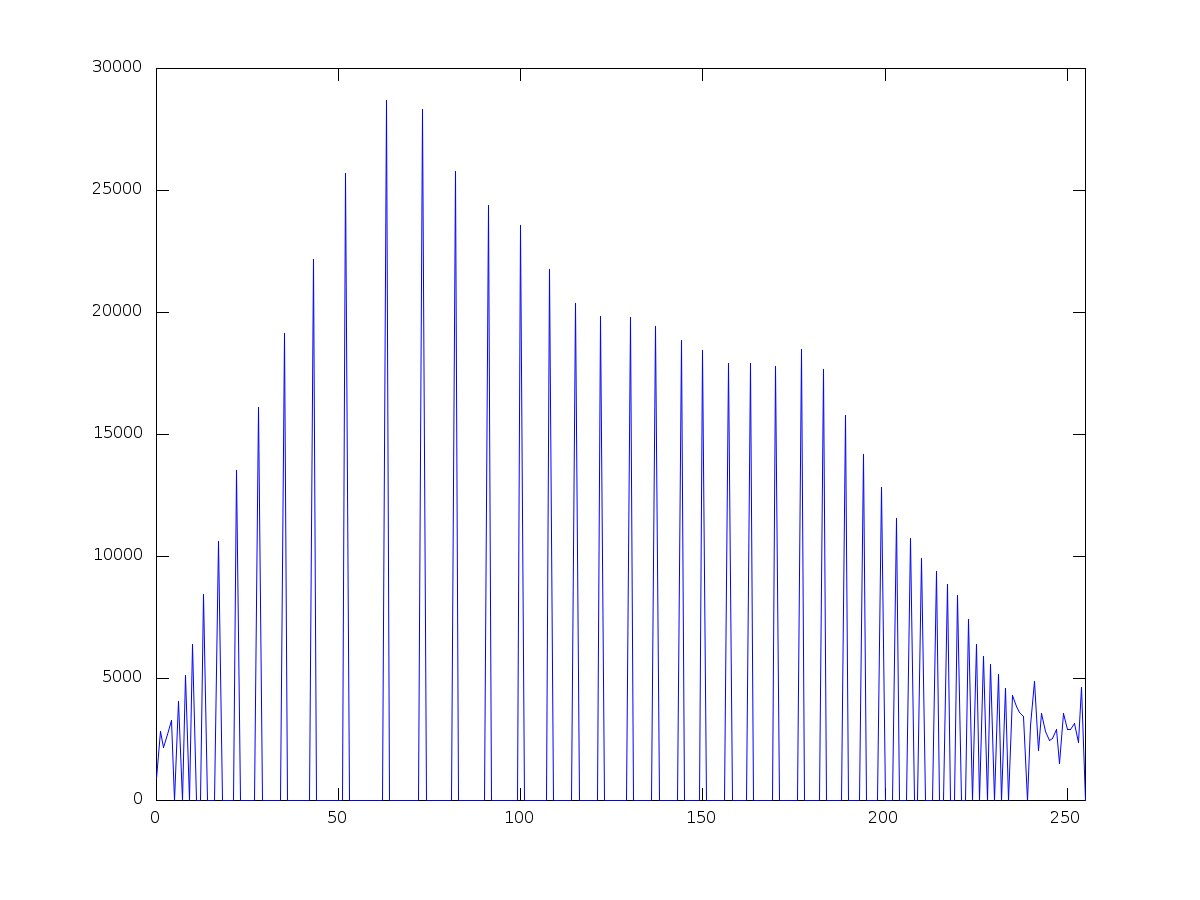
\includegraphics[scale=0.15]{imagens/hawkes-hist-novo.jpg}\\
			\hline
			\end{tabular}
			\label{tab:gt}
			\end{table}

	\section{Filtros por Convolução}
		Há uma classe de filtros aplicáveis em imagens, tais como os que serão apresentados a seguir, que são filtros lineares. Tais filtros tem a característica que um pixel após a filtragem é dado como uma combinação linear de seus vizinhos. Os coeficientes utilizados na combinação linear podem ser agrupados como uma matriz a qual se dá o nome de kernel. 
		O processo de aplicar a transformação a cada um dos pixels da imagem fazendo uso do kernel é chamada de convolução. Fazendo uso da fórmula fornecida no enunciado, foi implementada uma função de convolução que dada uma imagem e um kernel primeiramente cria uma borda de zeros em torno da imagem original e em seguida aplica a combinação. O efeito é que a imagem resultante tem o mesmo tamanho da original. A função assim, tem o mesmo comportamento de \texttt{filter2(kernel, imagem, "same")} da biblioteca padrão do Octave/Matlab.
		A vantagem de utilizar convoluções é que fica possível aplicar qualquer transformação linear de maneira bastante simples, bastando apenas definir o kernel correspondente. Transformações lineares são muito variadas, há as translações, suavizações, remoção de ruído, aumento de nitidez, detecções de borda, etc.
		A desvantagem de filtragens por convolução é que a quantidade de operações para a filtragem é maior que no caso anterior. Agora, para determinar cada pixel é necessário $n \times m$ operações de multiplicação onde $n$ e $m$ são as dimensões do kernel.
		
		\subsection{Implementação}
\begin{lstlisting}
function [C] = aplicar_convolucao(A, K)
    [m_A, n_A] = size(A);
    [m_K, n_K] = size(K);
	
	borda = zeros(m_A + 2, n_A + 2);
	borda(2 : m_A + 1, 2: n_A + 1) = A;
	A = borda;
	m_A += 2;
	n_A += 2;
	
    C = zeros(m_A - m_K + 1, n_A - n_K + 1);

    for i = 1 : m_A - 2
        for j = 1 : n_A - 2
            C(i, j) = sum(sum(A(i : i + m_K - 1, j : j + m_K - 1) .* K));
        endfor
    endfor
endfunction

\end{lstlisting}


	
	\section{Filtro de Suavização por Média Ponderada}
		Este filtro cumpre sua função de suavizar uma imagem dada fazendo com que cada pixel da nova imagem seja uma média ponderada de todos os seus pixels vizinhos, atribuindo pesos distintos a cada um deles. 
	
		\subsection{Vantagens e desvantagens}
		
		\subsection{Implementação}
		
		\subsection{Testes realizados}

	%No método de aumento de nitidez, apresente também a imagem intermediária resultante da aplicação do operador Laplaciano.
	\section{Filtro de Aumento de Nitizez - Sharpening}

		\subsection{Testes realizados}


\chapter{Conclusão}
	O trabalho ajudou a fixar os conceitos vistos em aula, além de nos fazer entrar em contato com uma área não habitualmente abordada na graduação, Processamento de Sinais. Os alunos tiveram um contato prático com os conceitos, com a teoria relacionada sendo estudada à medida que havia necessidade de interpretar os resultados obtidos. Isso permitiu acumular diversos conhecimentos úteis enquanto resolve-se um problema real na área de Computação Musical. Ainda, a possibilidade de utilizar uma linguagem voltada pra processamentos matemáticos, tal como Octave, a escolhida para este trabalho, simplificou problemas de implementação, permitindo aos alunos focarem nos algoritmos propriamente ditos. Vencida a dificuldade com o entendimento do problema a ser resolvido e questões de representação de números de ponto flutuante e complexos o EP foi bastante interessante de ser implementado.
	
\nocite{*}
\bibliographystyle{abnt-num}
\bibliography{bibliografia}
\end{document}

\end{document}
